%**********************************************************
\section{Tools Setup}
Before doing the system configuration it is necessary to first setup all of the used tools, as will be next presented.

%**********************************************************
\subsection{Git}
In order to make collaboration easier, allowing change by multiple people to all be merged into one source, Git will be used. Git is the most commonly used version control system. Before using it, it is necessary to do the correct setup as shown bellow.
\begin{lstlisting}
$ sudo apt install git
$ git config --global user.name "John Doe"
$ git config --global user.email johndoe@example.com
$ git config --global core.editor subl
$ cd ~
$ git clone git@github.com:ESRGgroup9/slipad.git
\end{lstlisting}

With this steps, Git is installed in a local machine, username and user email is defined alongside with the default core editor. After this, one can clone the repository for this project, created in GitHub, by executing line 6.

%**********************************************************
\subsection{Buildroot}
Buildroot is a simple, efficient and easy-to-use tool used to generate this project's embedded Linux system, through cross-compilation. The steps in order to install Buildroot in a local machine is shown bellow.

\begin{lstlisting}
$ cd ~
$ mkdir buildroot
$ cd buildroot
$ wget https://buildroot.org/downloads/buildroot-2021.02.5.tar.gz
$ tar xzf buildroot-2021.02.5.tar.gz
$ cd buildroot-2021.02.5
\end{lstlisting}

After the installation is done, one can do the base configurations, essential to the support the rest of the configurations.
\begin{lstlisting}
$ make raspberrypi4_defconfig
$ make menuconfig
$ make xconfig
$ make 
$ make clean
\end{lstlisting}

The first command is used to configure a kernel image for the Raspberry Pi 4, as it does the necessary configurations regarding hardware handling along with fetching some board specific packages. Then with the second and third commands, one can generate the graphic interface seen in figure \ref{fig:menuconfig}, presenting several sub-menus. 

\begin{figure}[H]
	\centering	
	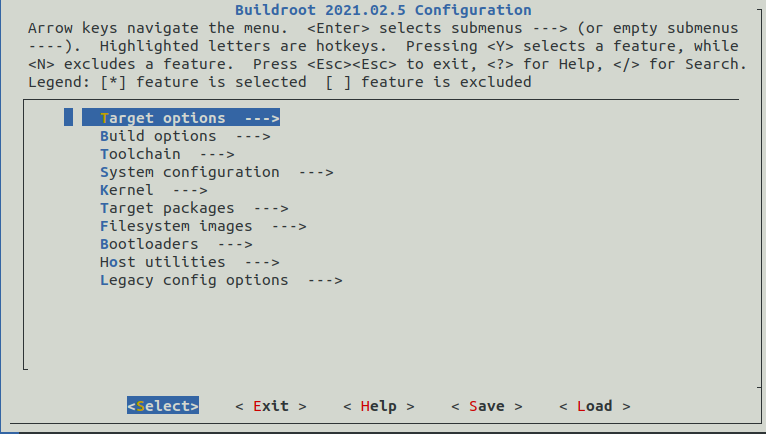
\includegraphics[width=.74\textwidth]{11configs/menuconfig}
	\caption{Buildroot menuconfig.}
	\label{fig:menuconfig}
\end{figure}

%**********************************************************
\subsection{OpenCV}

\begin{lstlisting}
$ cd ~/buildroot/buildroot-2021.02.5/output/build/opencv3-3.4.13/buildroot-build
$ cmake-gui
$ cmake .
$ make -j8
$ sudo make install
\end{lstlisting}

%**********************************************************
\subsection{Qt Creator}

The Qt Creator IDE was used to create an application that is used by the operator to interact with the system. The IDE instalation is done by downloading the open-source online installer present on the official site, in the download page \cite{qt_creator}. In the figure \ref{fig:qt_instalation} is shown all the packages installed for this IDE.

\begin{figure}[H]
	\centering	
	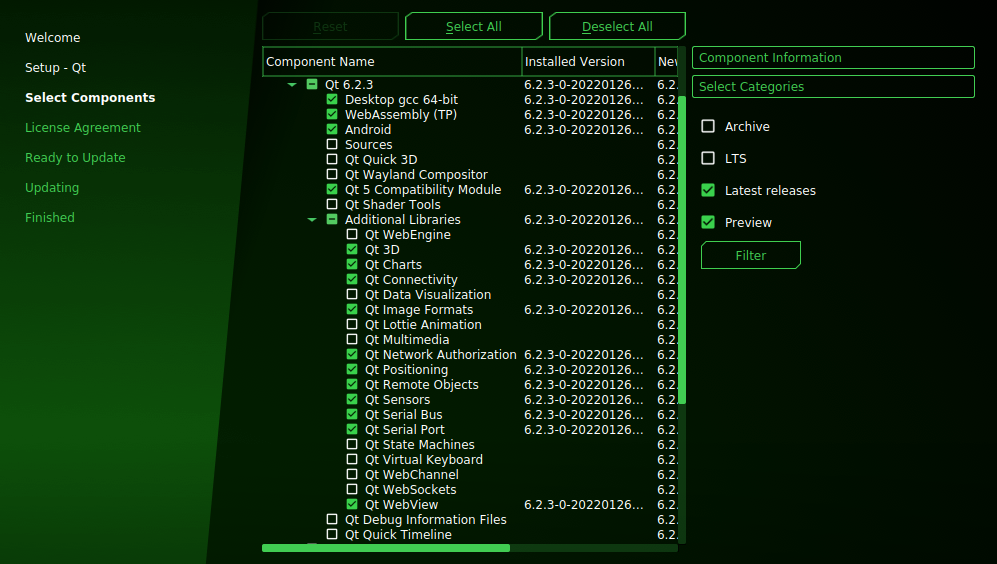
\includegraphics[width=.80\textwidth]{11configs/qt_instalation}
	\caption{Qt Creator: Instalation.}
	\label{fig:qt_instalation}
\end{figure}

Since one is deploying the application to an Android device, it was necessary to install and configure the Android Studio and SDK tools \cite{android_studio}, and also Android NDK \cite{android_ndk} in the Qt Creator. To install the Android Studio run \verb|<path-to-android-studio>/android-studio/bin/studio.sh|. Next, one needs to configure the platform of the Android Studio accordingly to the android phone version. The Android NDK must be the \verb|r23| version, and the Qt creator configure the packages missing.

It is also necessary to install a Java SE Development (JDK) \cite{java}. The JDK version shouldn't be the latest and the installed one was the version 11. Now, run \verb|<path-to-android-studio>/android/tools/bin/sdkmanager --licenses| in order to accept the licenses. 

At last, the \verb|QT -> Tools -> Options -> Devices -> Android|, sould look like shown in figure \ref{fig:qt_config}.

\begin{figure}[H]
	\centering	
	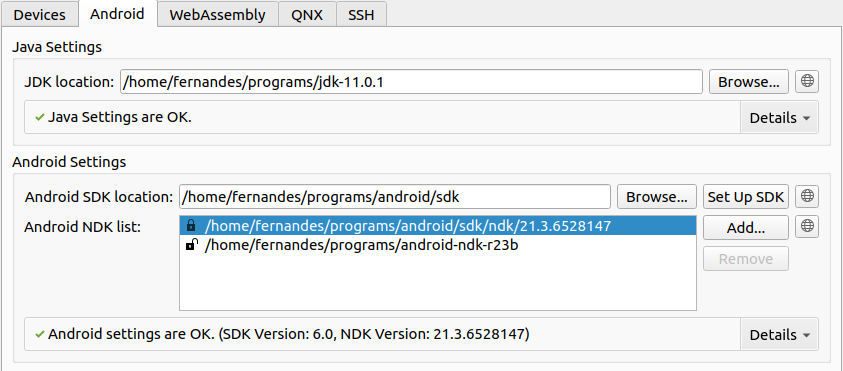
\includegraphics[width=.80\textwidth]{11configs/qt_config}
	\caption{Qt Creator: Configuration.}
	\label{fig:qt_config}
\end{figure}

%**********************************************************
\subsection{MySQL}
In order to have a fully managed database service to deploy cloud-native applications as MySQL, one has to firstly install it properly, as shown bellow.

\begin{lstlisting}
$ sudo apt-get install libmysqlclient-dev
\end{lstlisting}

First time runnning \verb|mysql|, one can create a strong password for \verb|mysql| access. After that, one can login into \verb|mysql| by typing:

\begin{lstlisting}
$ mysql -u root -p
\end{lstlisting}

%**********************************************************
\subsection{PHP}
In order to fetch data from the remote server database to the website that will present available parking spots, one uses PHP, which must first be configured. The following commands must be executed so that one gets a PHP client and PHP with MySql.

\begin{lstlisting}
$ sudo apt install php7.4-cli
$ sudo apt install php-mysqli
\end{lstlisting}

Knowing that fetching data from a remote database envolves secret keys, such as servername, username, port number, database password, it is usefull to have a \verb|.env| file which will contain all of them. In order to load those variables into the website index file one needs to setup \verb|phpdotenv| following the steps bellow. \cite{phpdotenv}

\begin{lstlisting}
$ sudo apt install composer
$ composer install
$ composer require vlucas/phpdotenv
\end{lstlisting}

%**********************************************************
\subsection{Google Maps Credentials}
In order for the website to present the parking spaces at a given location in a map, one uses Google Maps API. In order to generate a Google API key, one needs to go to Google API Console \cite{googleapi} and:

\begin{enumerate}
	\item Create a \textbf{new project};
	\item In API Manager go into \textbf{Library} and select \textbf{Google Maps Javascript API};
	\item Select the created project to enable APIs;
	\item Enable API;
	\item In API Manager go into \textbf{Credentials} and in \textbf{Create Credentials} click \textbf{Create API key}	
\end{enumerate}

After this steps, one may retrieve the generated key and use it within website source file. Make sure that this does not leak since it is a secret key that it is not meant be shared.

%**********************************************************
\clearpage
\section{System Configuration}
\label{systemConfig}

In the Buildroot, using \verb|make menuconfig| one can use a graphic interface (as previously shown in figure \ref{fig:menuconfig}) to select packages and change configurations in order to create a custom linux image.\\

Under \verb|Target-Packages| select:
\begin{itemize}
%	\item \verb|Development tools|, select:
%	\begin{itemize}
%		\item \verb|git|
%	\end{itemize}
	
	% *****************************************************************************
	\item \verb|Networking applications|, select:
	\begin{itemize}
		\item \verb|arp-scan|: scan the network of a certain interface for alive hosts;
		\item \verb|arptables-legacy|: set up and maintain the tables of ARP rules;
		\item \verb|dhcpcd|: open source DHCP client;
		\item \verb|dropbear|: small SSH server which will let us log in remotely;
	\end{itemize}
	
	% *****************************************************************************
	\item \verb|Hardware Handling|
	\begin{itemize}
		\item \verb|spi-tools|: tools needed to use SPI. Used for LoRa module communication;
		\item \verb|i2c-tools|: tools needed to use I2C. Used for light sensor module, TSL2581;
		\item \verb|rpi-userland|: Used to detect camera hardware;
	\end{itemize}
	
	% *****************************************************************************
	\item \verb|Libraries|, select:
	\begin{itemize}
		% *******************************
		\item \verb|Hardware Handling|
		\begin{itemize}
			\item \verb|bcm2835|: C library for Raspberry Pi user programs;
			\item \verb|libv4l|: select \verb|v4l-utils tools|: API for real time video capture;
		\end{itemize}
		
		% *******************************
		\item \verb|Graphics|
		\begin{itemize}
			\item \verb|OpenCV3|: select \verb|jpeg support|, \verb|png support|, \verb|v4L support|, \verb|videoio|, \verb|highgui|, \verb|imgcodecs|, \verb|imgproc|, \verb|v4l support|: Used for image capturing and processing;
		\end{itemize}
	\end{itemize}

	% *****************************************************************************
	\item \verb|Audio and Video Applications|, select:
	\begin{itemize}
		\item \verb|v4l2grab|: utility for grabbing JPEG images;
	\end{itemize}
	% *****************************************************************************
	
\end{itemize}

%**********************************************************
\clearpage
\section{Image Generation}
After all the necessary tools, packages and configurations are done, one needs to finally create the Linux custom image, that will run on the Raspberry Pi.

\begin{lstlisting}
$ cd ~/buildroot/buildroot-2021.02.5/
$ make
\end{lstlisting}

After that one can copy the image into the SD card, that will go into the Raspberry Pi. For that one can use the linux \verb|dd| command. \cite{dd}

\begin{lstlisting}
$ sudo dd if=./output/images/sdcard.img of=/dev/sdb
\end{lstlisting}

With this command, one must define the input file, \verb|if|, which is the linux image, and the output file, \verb|of|, which is the SD card, being in this example named \verb|sdb|.


%**********************************************************
%\clearpage
\section{System Initialization}
The Buildroot generates the boot configuration, in the \verb|/boot/config.txt| file that contains system configuration parameters that are read when the system boots from the microSD card, and that would traditionally be edited and stored using a BIOS. \cite{configtxt} The listing \ref{lst:configtxt} shows the boot configuration file. For this project, one added the parameter in line 24, in order to enable the I2C device, the parameters in lines 26 and 27, to activate the camera.

\begin{lstlisting}[caption={/boot/config.txt file.}, label={lst:configtxt}]
# We always use the same names, the real used variant is selected by
# BR2_PACKAGE_RPI_FIRMWARE_{DEFAULT,X,CD} choice
start_file=start.elf
fixup_file=fixup.dat

kernel=zImage

# To use an external initramfs file
#initramfs rootfs.cpio.gz

# Disable overscan assuming the display supports displaying the full resolution
# If the text shown on the screen disappears off the edge, comment this out
disable_overscan=1

# How much memory in MB to assign to the GPU on Pi models having
# 256, 512 or 1024 MB total memory
gpu_mem_256=100
gpu_mem_512=100
gpu_mem_1024=100

# fixes rpi (3B, 3B+, 3A+, 4B and Zero W) ttyAMA0 serial console
dtoverlay=miniuart-bt

dtparam=i2c_arm=on 		# enable i2c

start_x=1             	# enable camera
gpu_mem=128           
\end{lstlisting}

%**********************************************************
\subsection{Init Scripts}
\verb|/etc/init.d| is a directory containing initialization and termination scripts for changing init states. File names in this directory are of the form \verb|[SK]nn<init.d filename>|, where \verb|S| means start this job, \verb|K| means kill this job, and \verb|nn| is the relative sequence number for killing or starting the job. \cite{initScript} For this reason, one must create a script, with name started by \verb|S|, inside \verb|/etc/init.d| in the Raspberry Pi, using for that, \verb|vi|.

In order to guarantee that each program is running after the system boots up, its necessary to create the respective init scripts, following the procedure detailed in listing \ref{lst:initScript}.

\begin{lstlisting}[caption={Procedure for creating an init script, named Sscript\_name}, label={lst:initScript}]
$ cd /etc/init.d
$ vi S<scriptName>.sh
$ chmod +x S<scriptName>.sh
\end{lstlisting}

The local system has the init script detailed bellow, in listing \ref{lst:lsScript}. This script must insert all necessary device drivers in order to correctly execute the local system's daemon, dSensors, and the main process. 

\begin{lstlisting}[caption={Init script for local system.}, label={lst:lsScript}]
#!/bin/sh

# Inserting i2c-tools
modprobe i2c-bcm2835
modprobe i2c-dev

# Inserting PIR DDriver
insmod /etc/pir.ko

# Inserting lampf DDriver
insmod /etc/lampf.ko

# Run local system's daemon sensor and main process
/etc/dSensors.elf &
/etc/localSys.elf
\end{lstlisting}

The gateway system has the init script detailed in listing \ref{lst:gatScript}. The gateway, \verb|gateway.elf| is connected via TCP-IP to the remote system. Therefore one can set the gateway to connect to \verb|10.42.0.1|, which is the network address of remote system in the same network as the gateway, in port \verb|5000|.

\begin{lstlisting}[caption={Init script for Gateway system.}, label={lst:gatScript}]
#!/bin/sh

etc/gateway.elf 10.42.0.1 5000
\end{lstlisting}

The remote system also has an init script, as shown in listing \ref{lst:rsScript}. This is responsible for running the website PHP server \cite{phpserver} and running the remote system in port \verb|5000|.

\begin{lstlisting}[caption={Init script for remote system.}, label={lst:rsScript}]
#!/bin/sh

# run website PHP server
php -S localhost:8000 -t ~/slipad/remoteSystem/website/ &

# run remote system
~/slipad/remoteSystem/bin/remoteSystem.elf 5000

\end{lstlisting}

%**********************************************************
\clearpage
\section{Device Drivers}
\subsection{tsl2581}
%.config - Linux/arm 5.10.1 Kernel Configuration
%> Device Drivers > Industrial I/O support > Light sensors
%
%-> TAOS TSL2580, TSL2581 and TSL2583 light-to-digital converters
%
%cat /lib/modules/5.10.1-v7l/modules.dep | grep tsl
In order to insert the \verb|tsl2581| device driver, available on the Linux kernel (\cite{code_tsl}) one needs to execute a series of steps.\\

Firstly, one needs to add a new entry on the Raspberry Pi device tree, regarding the \verb|tsl2581|. For that, one needs to change the Device tree Source file (.dts) for the Raspberry Pi, named \verb|bcm2711-rpi-4-b.dts|. This will be later compiled into a device tree binary (.dtb), when creating an image using Buildroot, which will be later passed by the boot loader to the operating system kernel. \cite{dtb}

\begin{lstlisting}
$ cd ~/buildroot/buildroot-2021.02.5/output/build/linux-custom/arch/arm/boot/dts
$ nano bcm2711-rpi-4-b.dts
\end{lstlisting}

At the end of the file, before \verb|__overrrides__|, the following code must be added, where \verb|reg| is the I2C address of the device. \cite{tsl2583_txt} 

\begin{lstlisting}
&i2c1 {
	status = "okay";
	
	tsl2581@29 {
		compatible = "amstaos,tsl2581";
		reg = <0x29>;
	};
};
\end{lstlisting}

For the Raspberry Pi, in the \verb|/boot/config.txt| file, one must enable \verb|i2c1| with a \verb|dtoverlay|, by adding the line of code shown next.
\begin{lstlisting}
dtoverlay=i2c1
\end{lstlisting}

When booting the Raspberry Pi, one must insert the \verb|tsl2581| device driver, but before that, some modules must be added using \verb|modprobe|.

This is an I2C based sensor, which uses the \ac{iio} interface. In order to provide the \ac{iio} API, needed in the device driver to be used, it is necessary to enable the \ac{iio} kernel subsystem, \verb|industrialio|. To enable the I2C bus, one must load the \verb|i2c-bcm2835| module. \cite{i2c_bcm2835}\\

After that, one can insert the \verb|tsl2581| device driver, \verb|ldr.ko|.

\begin{lstlisting}
$ modprobe industrialio
$ modprobe i2c-bcm2835
$ insmod ldr.ko
\end{lstlisting}

After the device driver insertion, one can use it to communicate with the sensor in order to acquire the ambient luminosity. For that, a “single” on-demand read can be issued by user-space directly by reading \linebreak \verb|/sys/bus/devices/iio:device/in_<type><index>_raw|. In this case, the \verb|read_raw()| callback should handle basically all the steps necessary to get the required measurement. \cite{read_tsl}
%**********************************************************
\subsection{PIR}

%**********************************************************
\clearpage
\section{LoRa communication}
LoRa communication was implemented by deriving a third-party software from Arduino. \cite{sx1278_lib} Using \verb|bcm2835| C library one was able to control all the needed GPIO and SPI functions. \cite{bcm2835} \cite{bcmspi}

By reading the LoRa module SX1278 documentation \cite{sx1278}, (page 80) one is able to find the figure \ref{fig:sx1278_spi}. The SPI interface gives access to the configuration register via a synchronous full-duplex protocol. One of three access modes to the registers is used - SINGLE access. In this mode:
\begin{itemize}
	\item \textbf{Write access:} an address byte followed by a data byte is sent;
	\item \textbf{Read access:} an address byte is sent and a read byte is received;
\end{itemize}

\begin{figure}[H]
	\centering	
	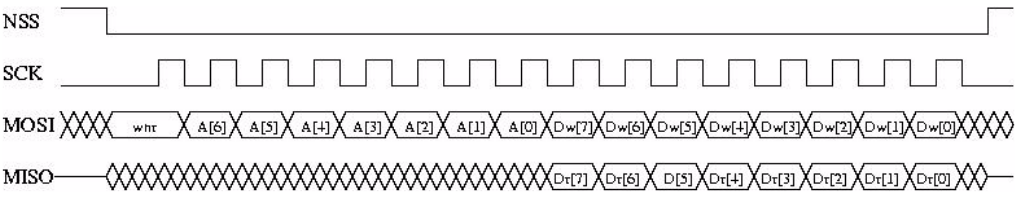
\includegraphics[width=1\textwidth]{12implementation/sx1278_spi}
	\caption{SPI Timing Diagram (single access).}
	\label{fig:sx1278_spi}
\end{figure}

A transfer is always started by the NSS pin going low. MISO is high impedance when NSS is high. MOSI is generated by the master on the falling edge of SCK and is sampled by the slave on the rising edge of SCK. MISO is generated by the slave on the falling edge of SCK. Both data to be transmitted and that has been received are stored in a configurable \ac{fifo} device. It is accessed via the SPI interface and provides several interrupts for transfer management. (Page 66, \cite{sx1278})
\\
In listing \ref{lst:lorasingletx} one can see LoRa single transfer function, which sends two bytes to the slave. 

\clearpage
\begin{lstlisting}[caption={LoRa single transfer.}, label={lst:lorasingletx}]
// set NSS pin low. Begin transfer
digitalWrite(_ss, LOW);

bcm2835_spi_transfer(address);
response = bcm2835_spi_transfer(value);

// set NSS pin high. Stop transfer
digitalWrite(_ss, HIGH);
\end{lstlisting}

By default, the device is configured at power up so that half of the available memory is dedicated to receive
(\verb|RegFifoRxBaseAddr| initialized at address 0x00) and the other half is dedicated for  (\verb|RegFifoTxBaseAddr| initialized at address 0x80). Therefore, when one wants to perform a transmit to the device, the address is always above \verb|0x80|. On the other hand, when one wants to perform a reading, the address is bellow \verb|0x80|. With that in mind one can use bit-masking to define the address for the operation, where, \verb|reg_addr| is the SX1278 register one wants to access:

\begin{itemize}
	\item \textbf{Read:} \verb|address = reg_addr & 0x7f| and \verb|value = 0x00|. The \verb|response| variable is the response from the slave;
	
	\item \textbf{Write:} \verb+address = reg_addr | 0x80+ and \verb|value| is the value to be written to the given address. \verb|response| is not used.
\end{itemize}

A LoRa message is defined by the class \verb|LoRaMsg| having the attributes shown in listing \ref{lst:loramsg}.

\begin{lstlisting}[caption={LoRa message.}, label={lst:loramsg}]
int recvAddr;     	// receiver address
int sendAddr;     	// sender address

int msgID;        	// message ID
size_t msgLength; 	// message length
string msg;       	// message
\end{lstlisting}

In listing \ref{lst:lorasend} is shown the main core of LoRa send function. This sends a series of attributes in each message, regarding destination address, sender address, message ID, message length and the message itself.

\begin{lstlisting}[caption={LoRa send function.}, label={lst:lorasend}]
beginPacket();

// add destination address  
write(destination);
// add sender address
write(localAddress);
// add message ID
write(msgCount);
// add message length
write(msg.length());
// add message
write(msg);

endPacket();
\end{lstlisting}

The function which implements LoRa receive, receives all of the attributes sent in the function above. Also it does some additional verifications to ensure communication integrity. The destination address in the message is compared to the local address of the device receiving the message, in order to avoid messages being mistakenly read. Besides that, one checks if the received message length matches the supposed length, by comparing the received message length to the message field regarding the message length.

In order to define LoRa status before a send/receive operation, a class is defined, as presented in listing \ref{lst:loraerr}.
 
\begin{lstlisting}[caption={LoRaError enum class.}, label={lst:loraerr}]
enum class LoRaError
{
	MSGOK = 0,  	// Message OK
	ENOADDR,		// Local address not defined
	ENOMSGR,    	// No message received
	ENOTME,     	// Message received is not for this device
	EBADLMSG    	// Message received lengths does not match
};
\end{lstlisting}

%**********************************************************
\clearpage
\section{PWM control}
In order to control the lamp, a PWM signal is used. For that, one can use \verb|bcm2835| library to control a PWM channel, producing the desired PWM signal at the selected GPIO pin. \cite{bcmpwm}

Considering that the clock which drives the PWM channels, \verb|clock|, is 54 MHz, and the lamp will operate at 50 Hz, \verb|freq|.

\[ RANGE = \frac{clock}{clock_{div} * freq} \]

Using a clock divider of 16, $clock_{div}$, one gets \verb|RANGE = 67500|. The variable \verb|RANGE| defines the maximum range of the PWM output, as shown in listing \ref{lst:pwmconfig}. One used \verb|PWM_CHANNEL 0|.

\begin{lstlisting}[caption={PWM configuration.}, label={lst:pwmconfig}]
// Set the output pin to Alt Fun 5, to allow PWM channel 0 to be output there
bcm2835_gpio_fsel(PWM_PIN, BCM2835_GPIO_FSEL_ALT5);
// set clock divider
bcm2835_pwm_set_clock(BCM2835_PWM_CLOCK_DIVIDER_16);
//CTL reg
bcm2835_pwm_set_mode(PWM_CHANNEL, 1, 1);
//RNG1/2 reg
bcm2835_pwm_set_range(PWM_CHANNEL, RANGE);
\end{lstlisting}

One can set the PWM pulse ratio to emit to \verb|RANGE|, where the duty cycle, \verb|duty| a value from 0 to 1, controls the PWM output ratio as a fraction of the range as shown in listing \ref{lst:pwmset}.

\begin{lstlisting}[caption={PWM set duty cycle.}, label={lst:pwmset}]
bcm2835_pwm_set_data(PWM_CHANNEL, (duty*RANGE));
\end{lstlisting}

%**********************************************************
\clearpage
\section{Luminosity Sensor}
\label{section:lumSensor}
As specified before, in order to know when to turn on/ off the lamp, it is used a luminosity sensor, the TSL2581. This module uses the I2C communication protocol to interface with the Raspberry Pi, being implemented based on a third-party software \cite{tsl2581_code}. As for the LoRa communication, one used the bcm2835 C library to communicate with the sensor module by I2C. \cite{bcmpiic}

From the theoretical foundations, one knows that the TSL2581 module uses a data line, SDA, to send and receive data, and a clock signal line, SCL, to synchronize the communication with the master device.

The sensor datasheet \cite{TSL2581_DS} shows that for the command code byte is used the \textit{Command Register} of the TSL2581, that is composed by:

\begin{itemize}
	\item \textit{CMD} bit: set to '1' when one wants to select the \textit{COMMAND} register;
	\item \textit{TRANSACTION} two bits: selects type of transaction to follow in subsequent data transfers, read/ write (R/W) mode and the special function register. For '00', select the I2C writing mode. For '10', selects the I2C reading mode which supports the read block protocol. For 11, select the special function register. 
	\item \textit{ADDRESS} five bits: when the \textit{TRANSACTION} field selects the R/W mode, then this field selects the bus address of the slave; when the \textit{TRANSACTION} field is set to '11', this field specifies a special command function.
\end{itemize}	

\myparagraph{I2C Address}

This module has three 7-bit address, as shown in table \ref{table:tsl_address}, and one can select one of them. By default, the \textit{ADDR state} register is set to FLOAT, so this device address in the I2C bus is the 0x39.

\begin{table}[H]
	\centering
	\begin{tabular}{|m{3cm}|m{3cm}|}
		\hline
		\textbf{ADDR State} & \textbf{Address}
		\\\hline\hline
		VCC & 0x49
		\\\hline
		FLOAT & 0x39
		\\\hline
		GND & 0x29
		\\\hline
	\end{tabular}
	
	\caption{TSL2581 I2C addresses.}
	\label{table:tsl_address}
\end{table}

\myparagraph{TSL2581 Initialization}

After connecting the device in the I2C bus, one should configure its registers before reading the value from its two ADC channels. In the listing \ref{lst:tslConfig} is shown the TSL2581 device initialization. First, one needs to configure the I2C bus, using the \verb|DEV_ModuleInit| function, passing, by argument, the device address of the light sensor, \verb|ADDR_FLOAT| (0x39, default). Using the \verb|CONTROL| register, one can power on the device, that puts all registers to their default value, enabling the R/W transactions. As the day-night transition is slow, one does not need to read the luminosity value much frequently, so one can define the maximum integration time (688,5 ms). It is also important to define the gain of the sensor. This sensor supports gains of 1, 8, 16 or 111. For indoor tests, it was used a gain of 16, but in a real outdoor model, it must be used a gain of 1.

\begin{lstlisting}[caption={TSL2581 Initialization.}, label={lst:tslConfig}]
if(DEV_ModuleInit(ADDR_FLOAT)==1)
	return false;

IIC_Write(COMMAND_CMD | CONTROL,CONTROL_POWERON);	// power on

IIC_Write(COMMAND_CMD | TIMING, INTEGRATIONTIME_688MS);  	// 688,5 ms
IIC_Write(COMMAND_CMD | CONTROL, ADC_EN | CONTROL_POWERON); // Every ADC cycle generates interrupt
IIC_Write(COMMAND_CMD | INTERRUPT, INTR_INTER_MODE);		// TEST MODE
IIC_Write(COMMAND_CMD | ANALOG, GAIN_16X);					// GAIN = 16
\end{lstlisting}

\myparagraph{Read Luminosity Values}

When the device is configured, one can read the luminosity values of the module channels. The TSL2581 has two channels: 

\begin{itemize}
	\item Channel 0: Value of visible and infrared light;
	\item Channel 1: Value of infrared light.
\end{itemize}

The listing \ref{lst:tslRead} presents the code that reads the channel 0 values, as for the channel 1 values, it is the same procedure. The lower byte is read out first using the \verb|DATA0LOW| register and next the higher byte, using the \verb|DATA0HIGH| register. Then, one combine them into a 16-bit variable as seen in the line 3.

\begin{lstlisting}[caption={TSL2581 Channel 0 read.}, label={lst:tslRead}]
DataLow = IIC_Read(COMMAND_CMD | TRANSACTION | DATA0LOW); 	// read channel 0 low byte
DataHigh = IIC_Read(COMMAND_CMD | TRANSACTION | DATA0HIGH);	// read channel 0 high byte
Channel_0 = 256 * DataHigh + DataLow ;
\end{lstlisting}

This values should be now converted to the luminous intensity. First, one needs to scale the value using the formula presented in the listing \ref{lst:tslscale}.

\begin{lstlisting}[caption={TSL2581 Channel 0 scaling.}, label={lst:tslscale}]
// scale the channel values
channel0 = (Channel_0 * chScale0) >>  CH_SCALE;
\end{lstlisting}

After scaling, it is calculated the ratio between channel 0 and channel 1 using the formula shown in listing \ref{lst:tslscale}.

\begin{lstlisting}[caption={TSL2581 ratio calculation.}, label={lst:tslratio}]
ratio1 = (channel1 << (RATIO_SCALE + 1)) / channel0;
ratio = (ratio1 + 1) >> 1; // round the ratio value
\end{lstlisting}

After calculate the multiple of the relative channel using the formulas given in the datasheet, one can export the current luminous intensity through the code presented in listing \ref{lst:tslCalc}, where lux is the final luminosity value. 

\begin{lstlisting}[caption={TSL2581 luminosity value calculation.}, label={lst:tslCalc}]
temp = ((channel0 * b) - (channel1 * m));
temp += (1 << (LUX_SCALE - 1));			// round lsb (2^(LUX_SCALE-1))
//  temp = temp + 32768;
lux_temp = temp >> LUX_SCALE;			// strip off fractional portion
\end{lstlisting}

%**********************************************************
\clearpage
\section{Database}
As previously stated, this system's database is developed using MySql. Analysing the two main entities of the database, \verb|lamppost| and \verb|location|, one can see its implementation in listing \ref{lst:locationLamppost}.

\begin{lstlisting}[language=SQL, caption={Queries to create tables location and lamppost.}, label={lst:locationLamppost}]
DROP TABLE IF EXISTS `location`;
CREATE TABLE `location`(
	`id` INTEGER AUTO_INCREMENT,
	`latitude` DECIMAL(8,6) NOT NULL,
	`longitude` DECIMAL(9,6) NOT NULL,
	`post_code` CHAR(8) NOT NULL,
	`street_name` CHAR(50) NOT NULL,
	CONSTRAINT `UC_Coords` UNIQUE (`latitude`,`longitude`),
	PRIMARY KEY(`id`),
	FOREIGN KEY(`post_code`) REFERENCES `region`(`post_code`)
		ON UPDATE CASCADE
);

DROP TABLE IF EXISTS `lamppost`;
CREATE TABLE `lamppost`(
	`id` INTEGER,
	`address` INTEGER UNIQUE NOT NULL,
	`status` ENUM('FAIL', 'OFF', 'ON', 'MIN') DEFAULT('OFF'),
	`gateway_sd` INTEGER DEFAULT(-1),
	PRIMARY KEY(`id`),
	FOREIGN KEY(`id`) REFERENCES `location`(`id`)
		ON UPDATE CASCADE
);
\end{lstlisting}

In table \verb|location| there are a set of attributes needed to identify a particular location. Each location instance is directly connected with the existence of a lamppost. That way, the primary key for the lamppost table references the primary key from \verb|location|, which is the location \verb|id|.

Each lamppost is connected to the remote system, and that way to the database, through a gateway. For that reason, each lamppost instance needs to contain the socket file descriptor of the TCP connection established by the gateway that is connected to that lamppost (local system).\\

As in lamppost table, in table \verb|parking_space| each row is linked to a unique lamppost, which is connected to a unique location. Considering that the number of vacants in each parking space is initialized as zero, there is only the need of creating a parking space by defining its \verb|id|. For that reason, a trigger is used to insert a parking spot, in table \verb|parking_space|, after an insertion in \verb|lamppost|, using the id of the inserted lamppost as the id of the parking space. In listing \ref{lst:triggerinspark} it shown the implementation of the trigger in question.

\begin{lstlisting}[language=SQL, caption={Trigger to insert a parking spot after lampost insert.}, label={lst:triggerinspark}]
DELIMITER $$

DROP TRIGGER IF EXISTS insert_parking$$
CREATE TRIGGER insert_parking
	AFTER INSERT ON lamppost
	FOR EACH ROW
	BEGIN
		INSERT INTO parking_space(id) VALUES(NEW.id);
END$$

DELIMITER ;
\end{lstlisting}

\subsection{Populating the database}
In order to populate the database faster one defined the queries format shown bellow, in listing \ref{lst:populatedb}.

\begin{lstlisting}[language=SQL, caption={Queries examples to populate database.}, label={lst:populatedb}]
INSERT INTO operator(id, name, password) VALUES
(NULL, 'Jonh', 'pass');

INSERT INTO region(post_code, operator_id, parish, county, district) VALUES
('9999-999', 1, 'Azurem', 'Guimaraes', 'Braga');

INSERT INTO location(id, latitude, longitude, post_code, street_name) VALUES
(1, 41.447986, -8.300469, '4800-045', 'Alameda Dr. Alfredo Pimenta');

INSERT INTO lamppost(id, address) VALUES
(1, 0xa2);

\end{lstlisting}


\section{Parking spots detection}
As previously stated before, the parking spots detection algorithm is based on OpenCv API. First one needs to capture a frame using the Raspberry Pi camera and store it, as shown in listing \ref{lst:captureframe}. 

\begin{lstlisting}[language=C, caption={Capture and Store frame from Camera.}, label={lst:captureframe}]
// read frame into lastFrame
camDev.read(lastFrame);

// write image to path
imwrite(IMAGE_PATH, lastFrame);
\end{lstlisting}

To capture the frame, one used the \ac{v4l} API and calibrated the camera parameters using the code present in listing \ref{lst:calibrateCamera}, in order to get a clear image from the camera. 

\begin{lstlisting}[language=C, caption={Capture and Store frame from Camera.}, label={lst:calibrateCamera}]
camDev.set(CAP_PROP_FRAME_WIDTH , FRAME_W); // 640
camDev.set(CAP_PROP_FRAME_HEIGHT, FRAME_H); // 480
camDev.set(CAP_PROP_BRIGHTNESS, CAM_BRIGHTNESS); // 20
camDev.set(CAP_PROP_CONTRAST, CAM_CONTRAST); // 0
camDev.set(CAP_PROP_SATURATION, CAM_SATURATION); //10

system("v4l2-ctl --set-ctrl=auto_exposure=0");
system("v4l2-ctl --set-ctrl=iso_sensitivity=4");
system("v4l2-ctl --set-ctrl=auto_exposure_bias=18");
system("v4l2-ctl --set-ctrl=exposure_time_absolute=1000");
system("v4l2-ctl --set-ctrl=exposure_dynamic_framerate=1");
system("v4l2-ctl --set-ctrl=white_balance_auto_preset=7");

system("v4l2-ctl --set-ctrl=sharpness=30");
\end{lstlisting}

When there is a image from the empty parking spots, one can identify the number of parking spots available for that lamppost. For that, it was used an algorithm that detect rectangles in an image since a parking spot shape is a rectangle. First, we apply the Gaussian blur to the image, in order to filter the image noise. Then, one searches for squares in every colour plane of the image, starting for mixing the channels an try several threshold levels with the canny edge detection function. After dilate the image to remove the holes between edge segments, one can find contours and store them in a list of 2D points. In the end, it is verified if the contours are between a defined size and if they don't overlap another rectangles. If the answer is affirmative, then contour is added to the park coordinates in the image held in the vector \verb|parkCoords|. In the listing \ref{lst:getOutline}, is shown the algorithm that detects parking spots in an image.

\begin{lstlisting}[language=C, caption={Parking Spots Detection.}, label={lst:getOutline}]
// apply gaussian
GaussianBlur(frame, gaussian, Size(7, 7), 0);

Canny(gray0, gray, 0, thresh, 5);
		
// find contours and store them all as a list
findContours(gray, contours, RETR_LIST, CHAIN_APPROX_SIMPLE);
	
// test each contour
for( size_t i = 0; i < contours.size(); i++ )
{
	addPark(contours[i]);
}
\end{lstlisting}

When one have the the parking spot outline, it is ready to detect if the parking spot is empty or vacant, using for that, the algorithm that detect objects from OpenCv using a Haar Cascade classifier, \verb|detectMultiScale|. It was used a pre-trained classifier to detect cars. If the centre of the detected car is near the centre of the parking spot than it means that the parking spot is occupied. In listing \ref{lst:detectCars}, is shown the algorithm that determines if the parking spots are empty or occupied. 

\begin{lstlisting}[language=C, caption={Empty Parking Spots Detection.}, label={lst:detectCars}]
vector<Point> rect = getRectPoints(features[f]);
	
// Is the car over the parking spot?
//  The center of the car match with the center of the parking spot?
int pos = isOverlapp(rect);
if( pos != -1 )
{
	vacantsNum--;
	// park unavailable
	parkStatus[pos] = 0;
}
\end{lstlisting}

\section{Website}

\section{Mobile Application}

The mobile application interacts with the database via TCP/IP via local server. When the application is executed, it tries to connect to the server held, in this case in the IP \verb|192.168.1.114| and port \verb|5000|. In the listing \ref{lst:appConnection}, is represented the connection establishment with the server. After the connection is done, the application sends a message to the server, indicating the type of its device, in this case, an application (\verb|TYPE;2|).

\begin{lstlisting}[language=C, caption={Mobile Application: Connection to the server.}, label={lst:appConnection}]
CTCPclient tcp(string("192.168.1.114"), 5000);

int main(int argc, char *argv[])
{
	// connect to tcp server
	ret = tcp.connect();
	if(ret == 0)
	{
		qDebug() << "Connection established";
		break;
	}
	
	err = errno;
	if(err != ECONNREFUSED)
	{
		// unexpected connection error
		qDebug() << "[CGateway::connect] Connect failed: " << err;
	}
	
	// send type to remote system
	QString msg = "TYPE;2";	
	do
	{
		ret = tcp.send(msg.toStdString());
		err = errno;
	} while((ret == -1) && (err == EAGAIN));
	
	// Handle errors
	...
}
\end{lstlisting}

When the operator tries to add a lamppost to the database, the application has to get the actual GPS location from the mobile phone. In the listing \ref{lst:appLocation} is shown the code that obtains the location from a \verb|QGeoPositionInfoSource|, connecting first to it and then start receiving updates in a period of 1 second. When the application wants to access the location, it can be done using the \verb|source->lastKnownPosition().coordinate()|, that return the last known position coordinates.

\begin{lstlisting}[language=C, caption={Mobile Application: Obtain GPS coordinates.}, label={lst:appLocation}]
source = QGeoPositionInfoSource::createDefaultSource(this);
if ( source )
{
	// conect to GPS
	connect(source, SIGNAL(positionUpdated(QGeoPositionInfo)), 
			this, SLOT(positionUpdated(QGeoPositionInfo)));
	// start updating localization
	source->startUpdates();
}
\end{lstlisting}

When a button is pressed in a window, it is executed the correspondent trigger function and when one wants to show other windows, it must be defined one instance of the window and call the \verb|show| function. In listing \ref{lst:appButton}, one can see an example of a button pressed call back function that invokes another window.

\begin{lstlisting}[language=C, caption={Mobile Application: Button trigger function.}, label={lst:appButton}]
void menu::on_add_new_released()
{
	addMenu = new addLamp(this);
	addMenu->show();
}
\end{lstlisting}
